\documentclass[letterpaper, 10 pt, conference]{ieeeconf}
%=======================================
%	Packages
%=======================================
%\IEEEoverridecommandlockouts
%\overrideIEEEmargins
% The following packages can be found on http:\\www.ctan.org
%\usepackage{graphics} % for pdf, bitmapped graphics files
%\usepackage{epsfig} % for postscript graphics files
%\usepackage{mathptmx} % assumes new font selection scheme installed
\usepackage{url} % assumes new font selection scheme installed
\usepackage{amsmath} % assumes amsmath package installed
\usepackage{amssymb}  % assumes amsmath package installed
\usepackage{graphicx}
\usepackage{color}
\usepackage{subfiles}
\usepackage{comment}
\usepackage[lined,ruled]{algorithm2e}
%=======================================
\title{A Self-Governing, De-Centralized, Extensible Internet of Powered Things}
%\author{\IEEEauthorblockN{Horia A. Maior}
%\IEEEauthorblockA{School of Computer Scienced\\
%Mixed Reality Lab\\
%University of Nottingham\\
%Email: psxhama@nottingham.ac.uk}
%\and
%\IEEEauthorblockN{Shrisha Rao}
%\IEEEauthorblockA{School of Computer Science\\
%International Institute of Information Technology\\ - Bangalore\\
%Email: Shirisha@iiitb.ac.in}}

\IEEEoverridecommandlockouts
\overrideIEEEmargins

%=======================================
%	Authors
%=======================================
%\numberofauthors{2}
%\author{
%% Horia Maior
%\alignauthor Horia A. Maior\\
%\affaddr{Mixed Reality Lab} \\
%\affaddr{University of Nottingham} \\
%\email{psxhama@nott.ac.uk}
%% Shirisha Rao
%\alignauthor Shrisha Rao\\
%\affaddr{IIIT-B} \\
%\affaddr{International Institute of Technology Bangalore} \\
%\email{Shirisha@iiitb.ac.in}
%}

\author{Horia A. Maior$^{1}$ and Shrisha Rao$^{2}$% <-this % stops a space
\thanks{$^{1}$Horia A. Maior, Mixed Reality Lab, Faculty of Computer Science, University of Nottingham, United Kingdom.
        {\tt\small psxhama@nottingham.ac.uk}}%
\thanks{$^{2}$Shrisha Rao, International Institute of Information Technology - Bangalore, India.
        {\tt\small srao@iiitb.ac.in}}%
}
\begin{document}

\maketitle
\thispagestyle{empty}
\pagestyle{empty}


%\bibliographystyle{acm-sigchi}%Choose a bibliograhpic style


\date{08 January 2014}

\begin{abstract}
  The Internet of Things is a term to describe networked objects not traditionally thought of as computers (e.g., cars, household appliances) which may nonetheless be connected using Internet protocols and technologies (TCP/IP, etc.). It is envisioned that an Internet of Things will be useful in particular in resource-constrained systems (e.g., with smart grids). The naive approach to an Internet of Things would use a central controller or master node of some sort to oversee the activities of all ``things'' in the Internet of Things. However, this has obvious drawbacks, not the least being scalability. It is therefore desirable that a ``thing'' govern its own actions while achieving global ``self'' properties in an Internet of Things that has to work with resource constraints (e.g., limited allowable peak electricity usage for a domestic or industrial system of many ``things''). Such an Internet of Things with self-governing ``things'' would not require a central controller, and addition or removal of ``things'' would be far easier. This paper provides a theoretical framework with a model of such Self-Internet of Things, giving a set of principles and properties to the system in respect to resource-constrain and energy efficiency systems. This would involve a proposed type of behaviour for a single ``thing'' in such an Internet of Things, as well as the principles or protocols by which such ``things'' are connected with one another.
\end{abstract}
%=======================================
%	Terms / Catagory / etc
%=======================================
% A category with the (minimum) three required fields
%\category{}{Internet of Things, Distributed systems}{Self-Stabilization}

%\terms{Evaluation Methods}
{\bf Keywords:} Internet of Things, Distributed Systems, Resource Allocation and Management.

%=======================================
%	Include Sections
%=======================================
\section{Introduction and Background}\label{intro}
\subsection{Self-governing, decentralized, extensible IoT, connected to a shared, variable power supply. Each thing is an object.}
A lot of effort is invested when comes to managing and distributing resources to large, almost implied distributed systems. A common resource of this type is the power resource; powering all kinds of ``things'' around us, such as households appliances (fridge, computer, toaster etc.), heating systems (e.g. of the house, of the office), etc. The Internet of Things (IoT) is a term to describe such networked ``things'', objects not traditionally thought of as computers (e.g. cars, household appliances), which may nonetheless be connected using Internet protocols and technologies (TCP/IP, etc.). Assuming such a network of objects, connected to a shared power supply, in this paper we are creating a framework for a Self-Governing, Decentralized, Extensible, Non-Preemptive IoT, where objects communicate and cooperate together to achieve system efficiency (in terms of power consumption).

The naive approach to the IoT would use a central controller or master node of some sort to oversee the activities of all objects of the system, and make decisions on behalf of the objects (e.g. decide when the toaster should be powered). The objects would then ``simply follow these instructions'' \cite{palattella2012standardized}. However, the approach has got clear limitations and drawbacks, not the least being scalability. We are talking about an extensible large system, where new objects can join the system at any point. One other issue may be the reliability of the system. If \emph{the single point of failure (SPOF)} exists, the entire system would stop working, and all objects of the system would fail to get powered.

A decentralized approach however, would better fit the needs of such IoT, overtaking the limitations mentioned above. All objects of the system would required to have a controller of some kind, which provides them with computing capabilities. This would make them capable of making own decisions, therefore let us call them self-governing objects. Liu and Zhou \cite{IoT6150221} describes such property as ``autonomy Feature'' of objects, where objects have the ability to reason, negotiate, understand, adapt and learn from other objects or environments. Such an Internet of Things with self-governing ``things'' would not require a central controller, and addition or removal of ``things'' would be far easier.

\subsection{Prioritized objects, cooperating and creating individual views of the system}
We described an IoT system where objects are interconnected, and in the same time connected to a power supply. Each object of the system consumes an amount of power resource, that can be different from object to object (e.g. a toast will consume less power than a washing machine). We assume this amount to be constant for each object, that means each object consumes a fixed amount of power or none, and this amount cannot change in time.

The power supply is something that supplies the system with power resource. In the real world, if we think of power suppliers, they might provide a variable amount of power budget, that means at different times there is different power resource available (e.g. thinking of a wind turbine, the provided power resource would be dependant on how much wind there is). Therefore, we assume the power resource to be variable in time and dependent on some external factors. We will also assume that there is only one power supply in the IoT system.

The total demand of system at any one time (regardless of resource), as described by Rao~\cite{rao2011foundation}, is the sum of all resource demands for all processes in a system. In our case, the total demand of power resource is the sum of all power demands of all objects in the system. One question is, what happens if the total demand of the system exceeds the power resource provided by the power supply. The answer is we cannot satisfy all objects with power. We are assuming that we cannot partially fulfill an object with power. It is either powered, therefore it consumes the fixed amount of power demand it requested, or not powered and consumes nothing. Rao~\cite{rao2011foundation} describes that in practice, distributed processes (objects in our case) drawing some sort of resource (power resource in our case), are distinguished from one another in terms of some sort of priorities. This is because some objects are more important than others in terms of their functions and utilities, and if the power supply cannot satisfy all the objects, priority will distinguish between which objects should be powered with the available power resource. Following the presented approach, objects with higher priority will be provided with power resource first (See Figure \ref{fig1})
\begin{figure}[h]
  \centering
  % Requires \usepackage{graphicx}
  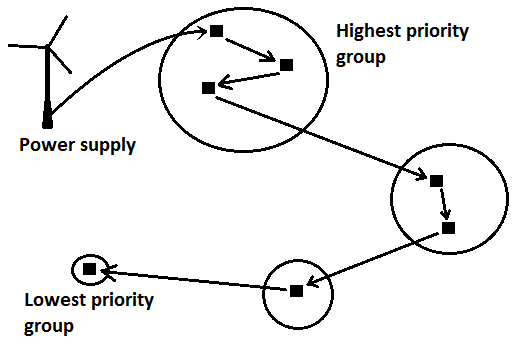
\includegraphics[width=80mm]{model.png}\\
  \caption{The flow of powering the system after priorities.}\label{fig1}
\end{figure}

Not having a central controller, all objects of the system need to decide when it is a suitable time for them to get powered. Therefore, they need to have a general overview of their position in the system in terms of their priority compared to other objects priorities and their power demand compared with other objects power demand. They achieve this by communicating and informing other objects about their details, while receiving information from all the other objects.

All the objects in our IoT framework are connected, networked between them such that any object in the system can communicate - send or receive a message - with/from any other object in the system. Prasad and Kumar \cite{prasad2012energy} describes this particular aspect of IoT as the advance version of Machine to Machine communication, where objects are exchanging information between them without a human intervention. When sending a message, we will later describe two types of destinations: one to one message (where the message is sent from one object to another specific object), and message broadcasting (where messages are broadcasted/flooded over all other objects in the system - see Algorithm \ref{flood} in the further section). For simplicity of the model, we make abstraction of how objects are connected.

We are describing a system with non-preemptive power policy; meaning that there is no partial fulfillment. When an object was allocated power resource, it is not interrupted until it has finished its demands, or there is a change in the available power resources. In other words, if a new object with high priority joins the system at some point and a low priority object has been allocated with power, the new object has to wait until the low priority object is leaving the system, or more power is provided by the power supply. In the same time, there should be no dependencies between objects except priorities. That is when the available power resource exceeds the total demand of the system, all objects of the system shall be powered, and no object shall wait for a different object to finish its demands or leave the system.

In this section we expressed our interest and presented the focus of this paper. In the following section we will cover the related work and the background information. In Section \ref{problem} we will define the model of IoT as discussed in Section \ref{intro}, we will develop a series of algorithms describing the behaviour of such model and we will prove the correctness of our approach. Section \ref{results} then, will be the Results Section, where we will present our work with a small example. The last part of this paper, Section \ref{discussion}, will be Discussion, Conclusion and Further Work section.

\section{Background and Related Work} \label{related}

In this section we will discuss the related work and background information close to our focus.

The IoT has the potential to be a great method for solving a demand-management problem. Higgins et al. \cite{higgins2011distributed} discussed ``a pathway'' to flexible power system automation. He proposed a new approach, based on ``distributed intelligence'' rather than ``traditional centralized control'', the system benefiting on many levels. We further considered Higgins approach by creating a decentralized distributed model of IoT, where power resource consumers can join and leave the system, and in the same time, they adapt automatically \cite{bookIoT}, when needed (either a change in power or when consumers are joining or leaving the system).

One aspect of the IoT, Zorzi et al \cite{zorzi2010today} points out, is a first time opportunity to interact with the surrounding environments and to exchange information that previously was not available. He points out a series of issues when comes to IoT paradigm including connectivity, scalability, self-management capability, and energy management. In this paper we answer some of the issues addressed by Zorzi, and create a connected, extensible IoT, where objects are ``smart things'' with self-governing capabilities to apply it within energy management problem. Monnier \cite{whitePaper} discusses how the objects around us need to be more and more connected and he says that ``connectivity is the key to automation''.

Niyato et al. \cite{niyato2011machine} presents a system that is using M2M communication for optimizing and minimizing the costs of a home energy management system. He describes a smart grid system in three major parts: power generation, power distribution and power consumption. In the system described, the M2M communication is between the home appliances and the smart meters, and the whole system is still dependent on a central node (Control center \cite{niyato2011machine}). The approach we take here is overcoming the limitation of using a central controller of any sort. The objects in our model are using some sort of M2M communication, however in a different context. Objects (e.g. home appliances) are communicating between them rather than to the smart meters, and based on the whole system information they decide their own actions (e.g. when is a suitable consumption time). Karnouskos \cite{karnouskos2010cooperative} supports this approach, and points out that communication between objects and other entities (such as ``... alternative energy resources which are smaller and decentralized'') is a way to ``achieve common goals such as energy efficiency''. Walczak et al. \cite{walczak2012machine} also describes the M2M communication as part of the IoT and the Future Internet Engineering.

The combination of intelligent consumers and providers of energy, have been recently combined into The Internet of Energy. Bui et al. \cite{bui2012internet} presents a set of advantages of the combination smart grid - IoT such as decentralization of the control procedures (the approach we are taking in this paper). Bui mentions that from a communication perspective, the smart grid distribution network must also be scalable, hence the high number of devices that are assumed to take part in the future Internet of Energy.

Siano \cite{siano2014demand} is presenting ways in which the system can lower peak demand. On the other hand, in our system, we are considering the use of the power resource to the maximum possible. If we consider sustainable energy power source, the power available to the system has peaks, and it should be used to the maximum as possible at all times. Gelazanskas and Gamage \cite{gelazanskas2013demand} proposed a novel electricity demand control technique using real-time pricing. However, in this paper we do not consider pricing; instead, the focus of the paper is having a variable in time power budget(thinking of a solar power provider, during daytime there will be more power available to consume compared to night time).

In this section we introduced the topic and presented an overview of our interest. The following section is to describe the framework of IoT by creating a model of such system, developing some algorithms for the distributed IoT, and at the end presenting and developing some profs of correctness of our work.



\section{Problem Statement and The Model}\label{problem}
In Section \ref{intro} we discussed and presented our interest and in the same time the focus of this paper. In this section we will describe an abstract model of IoT within resource-constrained domain, formally stating the problem we address. We will develop algorithms working on the model developed and we will attempt to prove the correctness of the main properties of our system.

\subsection{Definition and Notations}
Let there be numerous objects $o_{i}$ that demand and may consume power resource. The set of all objects, denoted as $O$, together with some sort of power supply constitute the whole system.
 \begin{center}
    $O=\{o_{0}, o_{1}, ...,o_{n-1}\}$, the set of all $n$ objects.
 \end{center}
Each object consumes a non-negative amount of power resource. To simplify the system, let us consider this non-negative amount of power constant for each object in the system (an object cannot change its power demand). Let $\mathbb{R^+}$ be the set of positive real numbers, then let the demand function, $f:O\rightarrow\mathbb{R^+} | f(o_{i})=r$, give the power demand of each object $o_{i}$. This means object $o_{i}$ demands $r$ amount of power from the power supply.

The Total Demand of system at any one time, as described by Rao~\cite{rao2011foundation}, is the sum of all power demands for all objects in the system:
\begin{center}
  %$\sum_{i=0}^{n-1} o_i$
   $\sum\limits_{i=0}^{n-1} f(o_i)$
\end{center}

The power supply can be described as the total amount of power resource available to share between all the objects of the system at any time. The main property of the power supply is that it is variable in time. Let the set $T$ denote the set of all time instances, and $\mathbb{R^+}\cup\{0\}$ be the set of positive real numbers including $0$. Then, the function $\gamma:T\rightarrow\mathbb{R^+}\cup\{0\}$ denotes the power supply function. With $\gamma(t)= w$, $w$ the \cite{rao2011foundation} the maximum resource limit, in our case power resource, available in the system at a given time $t$.

We described objects having various power demands and we described a power supply providing the system with power resource. As presented in the introduction, objects also differ between them in terms of some sort of priority.

Let $\delta:O\times T\rightarrow\mathbb{R^+}\cup\{0\}$ be the priority function, with $\delta(o_{i}, t)= p$, where $p$ is the priority of object $o_{i}$ at time $t$. As described, priority function is time dependent, that means objects can change priority in time.

\subsection{IoT as a Distributed System}

In a distributed IoT, every object is networked in some way so it is able to exchange information with all other objects in the system (for simplicity, we make abstraction of how they are physically networked). It is also assumed that every object has some sort of computing capability (we assume that computing capability has no cost what so ever), and it is in some way `self-aware' of its current `needs' (for example each object knows or is able to find out about its power settings). Because we are building a de-centralized system, the decision-making comes to the object itself (this means that each object in the system decides on its own when is a suitable time to consume power resource), therefore, every object is also interested in an overview of the whole system (for example each object needs to know the maximum power limit $\gamma(t)= w$ but also each object has to know about what is its priority relative to other's in the network).

When creating such a system, each object in the system is ``exploring'' the whole system in some way. During the exploration, objects need to find out (and memorize in some way) other objects with the same priority, and in the same time find out other priorities in the system. This way, every object will have an general overview of what is their own priority relative to other object in the system. The exploration is possible trough some sort of communication and exchange of information between objects. Making abstraction of how the communication is made, let $v$ and $u$ be two objects; $v,u \in\{O\}$. Let $msg(v,u,m)$ be a message, where $v$ is the sender of the message, $u$ is the delivery object of the message and $m$ is the message (the message can contain any kind of information coming from the sender). Following Peleg's approach \cite{peleg2000distributed}, a message can be also broadcasted or ``flooded'' to/over a network (in our case system). Algorithm \ref{flood} below, is an adapted version from \cite{peleg2000distributed}, for broadcasting a message across all $n$ objects of a system, from a root object $o_{j}$:

%Algorithm 1 - Flooding
\LinesNumbered
\IncMargin{1em}
\begin{algorithm}
%\DontPrintSemicolon
Let a source $o_{j}$
\BlankLine
\For{$i \gets 0$ \textbf{to} $n-1$} {
    \If {$i!=j$} {	
        \textbf{Send} \emph{$msg(o_{j},o_{i},m)$}
    }
}
\For{$i \gets 0$ \textbf{to} $n-1$} {
    \textbf{Upon} receiving a message $o_{i}$ \newline
       \textbf{Store} the message\newline
       \textbf{Compute} the message\newline
       \textbf{Send} acknowledgement
}
\caption{\textbf{Algorithm Flood}} \label{flood}
\end{algorithm}
\DecMargin{1em}

The number of messages sent by each object can be used to evaluate the complexity of the Algorithm \ref{flood} and all further algorithms developed in this paper. Each object running Algorithm \ref{flood} is sending a message to all other objects (in total $n-1$ objects); therefore the complexity of Algorithm \ref{flood} is $\mathcal{O}(n)$.

Using Algorithm \ref{flood}, we design an exploration algorithm that is run by all objects in the system, all trying to communicate to other objects information about their priority and their power demand. In the same time, objects receive, compute and store information about other objects. Therefore, every object will end up having an overview of their position in the system.

Let $o_{i}$ be an object; $o_{i} \in\{O\}$. As described above, each object stores information about other priorities in the system and other objects of the same priority in the system. Let each every object $o_{i}$ have to arranged lists:
\begin{itemize}
    \item let $P_{i}=$ be an arranged list where each object $o_{i}$ can store priorities of other objects (decreasing order); such that $P_{i}(0)$ is the highest priority in the set.
    \item let $Q_{i}$ be an arranged list of objects of the same priority as $o_{i}$ (increasing order); such that $Q_{i}(0)$ is the object with smallest demand.
\end{itemize}

Before joining the system and running the exploration algorithm, every object $o_{i}$ has: $P_{i}=\{\emptyset\}$ and $Q_{i}=\{\emptyset\}\cup\{\delta(o_{i},t)\}$. Please consider Exploration Algorithm (\ref{algo2})below.

%Algorithm 2 - exploration
\LinesNumbered
\IncMargin{1em}
\begin{algorithm}
%\DontPrintSemicolon
$t_{0} = current time$
\BlankLine
$o_{i} \gets$ Flood Algorithm over $G$ \newline
\textbf{Send}: $msg(o_{i}, join, \delta(o_{i}, t_{0}), f(o_{i}))$
\BlankLine
\For{$j \gets 0$ \textbf{to} $n-1$} {
    Let $o_{j}$, ($j!=i$) receive the message
    \BlankLine
    \textbf{Upon} receiving message:\newline
    \If {$\delta(o_{i},t_{0}) = \delta(o_{j},t_{0})$}
    {
       \textbf{Insert} $o_{i}$ in $Q_{j}$ \textbf{in order} of $f(o_{i})$
       \BlankLine
       \textbf{Send} acknowledgement ($\delta(o_{i},t_{0}) = \delta(o_{j},t_{0})$)
    }
    \Else {
        \If {$\delta(o_{i},t_{0}) \notin P_{j}$} {
            \textbf{Insert} $\delta(o_{i},t_{0})$ in $P_{j}$ \textbf{in order}
            \BlankLine
            \textbf{Send }acknowledgement $\delta(o_{i},t_{0}) < \delta(o_{j},t_{0})$ (if so) \newline
            \textbf{Send }acknowledgement $\delta(o_{i},t_{0}) > \delta(o_{j},t_{0})$ (if so)
        }
    }
}
\caption{\textbf{Exploration Algorithm} run by all object joining the system} \label{algo2}
\end{algorithm}
\DecMargin{1em}

The Algorithm \ref{algo2} has complexity $\mathcal{O}(n^2)$, and this is mostly because there are $n$ objects running the Algorithm \ref{flood}, every object sending $n-1$ messages (that is $n\times n$).

Being an extensible IoT system, new objects can join at any time, and objects may no longer want to be part of the system and leave at any time. An object joins the system when it demands power resource. When joining, the new object shall run the exploration algorithm. This way, other objects will make note of the new object's details (like priority and power setting), but in the same time, the new object will create it's overview of the system trough message acknowledgements from the existing objects. An object is leaving the system when it is no-longer interested in power resource at that particular time. On leaving, the object informs all the other objects about it's intentions.

Let $B = \{T,F\}$ the set of boolean values true ($T$) and false ($F$), and function $p:O\times T \rightarrow B$:

  \[ p(o_{i}, t)= \left\{
  \begin{array}{l l}
    $T$ & \quad \textrm{if $o_{i}$ is powered}\\
    $F$ & \quad \textrm{if $o_{i}$ is not powered}
  \end{array} \right.\]
When an object $o_{i}$ gets powered at time $t$, the boolean function $p(o_{i},t) \gets T$, becomes true. Algorithm \ref{algo3} below describes exactly what happens when an object is leaving the system.


%Algorithm 3 - removing an object
\LinesNumbered
\IncMargin{1em}
\begin{algorithm}
%\DontPrintSemicolon
$t = leaving time$
\BlankLine
$o_{i} \gets$ leave the system \newline
Flood Algorithm over $G$ \newline
\textbf{Send} $msg(o_{i}, leave,\delta(o_{i}, t), Q_{i}, f(o_{i}), powered=p(o_{i},t))$
\BlankLine
\For{$j \gets 0$ \textbf{to} $n-1$} {
    Let $o_{j}$, ($j!=i$) receive the message
    \BlankLine
    \textbf{Upon} receiving:\newline
    \If {$\delta(o_{i},t) = \delta(o_{j},t)$} {
          \textbf{Remove} $o_{i}$ from $Q_{j}$
    }
    \Else {
        \If {$Q_{i} - \{o_{i}\} = \emptyset$}{
            \textbf{Remove} $\delta(o_{i},t)$ from $P_{j}$
        }
    }
    \If{$powered = T$}{
        $w \gets w + f(o_{i})$
    }
}
\caption{\textbf{Leave Algorithm} run by every object leaving the system} \label{algo3}
\end{algorithm}
\DecMargin{1em}
On leaving, an object sends a message to all other objects in the system. Like Algorithm \ref{flood}, Leave Algorithm has the complexity $\mathcal{O}(n)$.

In Algorithm \ref{algo3}, the leaving object is messaging all other objects three important pieces of information:
 \begin{itemize}
   \item it's priority level $\delta(o_{i}, t)$ over (together with the list with other objects of it's priority $Q_{i}$)
   \item it's power demand $f(o_{i})$.
   \item whether or not the leaving object was powered (function $p(o_{i}$)).
 \end{itemize}

In the case that the leaving object has the same priority with the one receiving the message, the last one mentioned has to remove the the leaving object from the same priority objects database $Q_{j}$ (see line $5, 6$ in Algorithm \ref{algo3}). In the case that the leaving object is the last of its priority, the whole priority level is removed from the other priorities database $P_{j}$ (see line $9, 10$ in Algorithm \ref{algo3}). Finally, if the leaving object was powered, it's power demand becomes available for other objects (see line $13-15$ in Algorithm \ref{algo3}).

\subsection{Prioritized objects and a happy IoT}

In he subsections above, it has been described a distributed, extensible system, with objects that are able to communicate with other objects of the system, with new objects joining the system and objects maybe leaving the system. However, we did not yet mentioned how the system is powered from the power supply, that is how each individual object receives, if so, power resource.

We discussed that objects can have different priorities, and that is because some objects are more important in a way than others. In the case of not being able to satisfy all objects with power resource, higher priority objects are more likely to get power resource than lower-priority ones. We also discussed that objects can have different power demands. That is, one object might need more power resource than other ones. In the case of objects with the same priority level, the system shall always prioritize the low consumer object.

Let there be $n$ objects $o_{i}\in O$, with $0<=i<=n-1$. Each object has a power demand $f(o_{i})$, a priority function $\delta(o_{i}, t)$, and each object has created its own overview of other objects priorities in the system (in decreasing order the list $P_{i}$; such that $P_{i}(0)$ the highest priority), and objects with the same priority (in increasing order of power demands the list $Q_{i}$; such that $Q_{i}(0)$ is the smallest demand object of $o_{i}'s$ priority). The power supplies is denoted by the function $\gamma(t) = w$, providing the power resource available at every time $t \in T$. The following algorithm (Algorithm \ref{algo4}) describes how the power supplier, supplies the highest priority object with the smallest power demand first, and then how each object informs other objects about their actions and remaining power resource.

%Algorithm 4 - powering the system
\LinesNumbered
\IncMargin{1em}
\begin{algorithm}
%\DontPrintSemicolon
$t = current time$
\BlankLine
Let $o_{i}$ the object running this code
\BlankLine
\If {$\delta(o_{i}, t)>P_{i}(0)$ \textbf{and} $f(o_{i})=Q_{i}(0)$}{
    $w \gets \gamma(t)$
    \BlankLine
    \If{$f(o_{i})<=w$}{
        \textbf{Power} object $o_{i}$;
        $p(o_{i},t) \gets T$
        \BlankLine
        $w \gets w - f(o_{i})$
        \BlankLine
    }
    \If {$Q_{i} - \{o_{i}\} = \{\emptyset\}$}{
        $nextPriority \gets P_{i}(0)$
        \BlankLine
        \textbf{Broadcast} $msg(power, nextPriority, w)$
    }\Else{
        $nextObj \gets Q_{i}(1)$
        \BlankLine
        \textbf{Send} $msg(power, nextObj, w$)
    }
}
\textbf{Upon} receiving one of the msg:\newline
\textbf{Receiving} $msg(nextObj, w)$ or\newline
\textbf{Receiving} $msg(nextPriority, w)$\newline
\If{$(o_{i} = nextObj$)\textbf{ or }\newline
    $(\delta(o_{i}, t) = nextPriority$ \textbf{and} $f(o_{i})=Q_{i}(0))$}{
    \If{$f(o_{i})<=w$}{
        \textbf{Power} object $o_{i}$;
        $p(o_{i},t) \gets T$
        \BlankLine
        $w \gets w - f(o_{i})$\newline
    }
    \If {$Q_{i} - \{o_{i}\} = \{\emptyset$\}}{
        $nextPriority \gets P_{i}(j) <=>$ \newline
        $(P_{i}(j-1)>\delta(o_{i},t) > P_{i}(j)$)
        \BlankLine
        \textbf{Broadcast} $msg(nextPriority, w)$
    }\Else{
        $nextObj \gets Q_{i}(j) <=> (o_{i}=Q_{i}(j-1))$
        \BlankLine
        \textbf{Send} $msg(nextObj, w)$
    }
}
\caption{\textbf{Power Algorithm}} \label{algo4}
\end{algorithm}
\DecMargin{1em}

Algorithm \ref{algo4} is run by all objects in the system individually. The first part of the algorithm, lines $3-17$, will addresses to the object with the highest priority and the lowest power demand of the system (line $3$), this object having the first chance to get powered (in the case that the available power resource can satisfy its power demands - line $4-6$). From this point, the current object informs the next object with the same priority (if there is one - lines $13-16$), otherwise it broadcasts an information containing the new priority that shall receive power (lines $9-12$). The second part of Algorithm \ref{algo4}, lines $18-31$ address all the other objects of the system, which are waiting for a message addressing them or their priority level. The smallest consumer of a priority category will always be powered first. Regardless if an object gets powered, it will always send a message to the next object or priority group. This enables small demand objects with small priority to get powered in the case of a high priority object cannot fulfil its demands with available power resource.

The complexity of Algorithm \ref{algo4} is $\mathcal{O}(n^2)$. The worse case scenario is when all objects have different priorities, and every object is broadcasting a message once ($n\times n$).

\subsection{Proofs of Correctness}
In the previous subsections we developed a framework and created algorithms that describe the behaviour of objects within the IoT model. In this subsection, we are identifying a set of properties of the model, and we are trying to prove the correctness of our proposed design by validating these properties.
\newtheorem{theorem}{Theorem}[section]
\newtheorem{lemma}[theorem]{Lemma}
\begin{theorem}
\emph{No Wastage}. Guarantying that all the available power will be used by the objects of the system, and there will be not object entering a situation where there is available resource in the system meeting that objects demands but the object is not powered.
\end{theorem}

\begin{lemma}\label{lemma1}
  After running Algorithm \ref{algo4}, $\nexists o_{i}\in O, (p(o_{i},t) = F)$ \textbf{and} $(f(o_{i})\leq w); $
\end{lemma}

\begin{proof} Let us assume $\exists o_{i} \in O$ such that $p(i,t)=F$ while there is sufficient power to satisfy its demands, $(f(o_{i})\leq w)$. There are two cases to consider:

\begin{itemize}
  \item object $o_{i}$ is the highest priority object with the smallest power demand (between objects of the same priority); if $p(o_{i},t)=F$, following line $5,6$ in Algorithm \ref{algo4}, $(f(o_{i})\nleq w)$. Power demand $(f(o_{i})$ cannot be both $\leq\nleq w$. Hence the contradiction.
  \item Otherwise, object must have received a message from a higher priority object; in this case the proof is similar; if $p(o_{i},t)=F$, following line $19, 20$ in the same Algorithm \ref{algo4}, $(f(o_{i})\nleq w)$. Power demand $(f(o_{i})$ cannot be both $\leq\nleq w$.
\end{itemize}
\end{proof}


\begin{theorem}
\emph{No Priority Inversion}. Guarantying that high priority objects get powered first, if possible.
\end{theorem}
\begin{lemma}\label{lemma2}
      $\nexists u,v \in O$ such that ($\delta(u,t) \le \delta(v,t)$) \textbf{and} ($w\geq f(u)$ and $w\geq f(v)$), ($ p(u,t)=T$ \textbf{and} $p(v,t)=F$).
\end{lemma}

\begin{proof}
    If we assume $\exists u, v \in O$, such that priority of object $\delta(u,t) \le \delta(v,t)$ and the power budget can satisfy any of the two objects with power resource $w\geq f(u)$ and $w\geq f(v)$. We also assume that $p(u) = T$ \textbf{and} $p(v,t) = F$ after running Algorithm \ref{algo4} by both objects. There are two cases here:
    \begin{itemize}
      \item object $v$ is has the heights priority with the smallest power demand; following line $3-6$ in Algorithm \ref{algo4}, object $v$ gets powered first and $p(v,t) = T$. Object $v$ cannot be in the same time both powered $p(v,t) = T$ and not powered (the assumption of the proof) $p(v,t) = F$
      \item neither of the objects $u,v$ are the have the highest priority with the smallest power demand; objects get powered when receiving a message dedicated for them. Message flow is from the highest priority object (line $3$) towards the lowest priority object (line $9-16$). If , $p(u) = T$ and $p(v) = F$, the message must have first visited object $u$. Therefore $\delta(u,t) \ge \delta(v,t)$. But the priority comparison cannot be both $\delta(u,t) \le \delta(v,t)$ and $\delta(u,t) \geq \delta(v,t)$ in the same time. Hence the contradiction.
    \end{itemize}
    because the message flow (with the remaining power resource) starts from the highest priority object (line $3$) towards the lowest priority object (line $9-11$). Therefore the message with the remaining power resource must have first visited object $v$, therefore the contradiction.
\end{proof}

\section{Results} \label{results}
In the previous section we presented the framework of IoT in the context of energy efficient consumption. We created a model of the system and we developed a series of algorithms describing the behaviour of the objects in such a system. Towards the end of the section we attempted to prove the correctness of the model. This section is to present the results of our work with a simple pen and paper simulation example of the model described.

For this, we will take a sample of the IoT, consisting of objects from a ``smart'' house as consumers of power, and, by providing a limited power budget we will simulate which objects shall be powered. Each object will have a power demand (usage setting), that is the amount of power each object needs from the power supply, and also each object will have a priority (from 1 to 10) denoting their importance compared to other objects. The power resource is an amount of kilowatt $kW$ available to the consumers. In the same time, consumers consume $kW$ power resource. For notation purpose, in this sample, each object has the form \emph{ObjectName(NameAbbreviation, PowerDemand (kW), Priority)}.

Let the set of objects $O$ consists of (source of power consumption estimations for the household appliances \cite{bworld}): Electric Shower(ES, 7kW, 6), Dishwasher(Dw, 1.5kW, 1), Washing Machine(WM, 1.5kW, 2), Tumble Dryer(TD, 3kW, 2), Iron(Ir, 1.6kW, 2), Toaster(Ts, 1kW, 8), Oven(Ov, 2kW, 8), Grill(Gr, 1.8kW, 8), Fridge-Freezer(FF, 0.4kW, 10), Vacuum Cleaner(VC, 1kw, 3), Hairdryer(Hd, 1kW, 9), Plasma TV(TV, 0.4kW, 5), Desktop Computer(PC, 0.15kW, 9), Broadband Router(BR, 0.01kW, 10), and Smart Phone(SP, 0.005kW, 10).

After running Exploration Algorithm (Algorithm \ref{algo2}), each object knows where about in the system is compared to other objects priorities. Further, according to Algorithm \ref{algo4}, highest priority object with the smallest power consumption, will be powered first. Figure \ref{fig2} shows that SP should be powered first.
\begin{figure}[h]
  \centering
  % Requires \usepackage{graphicx}
  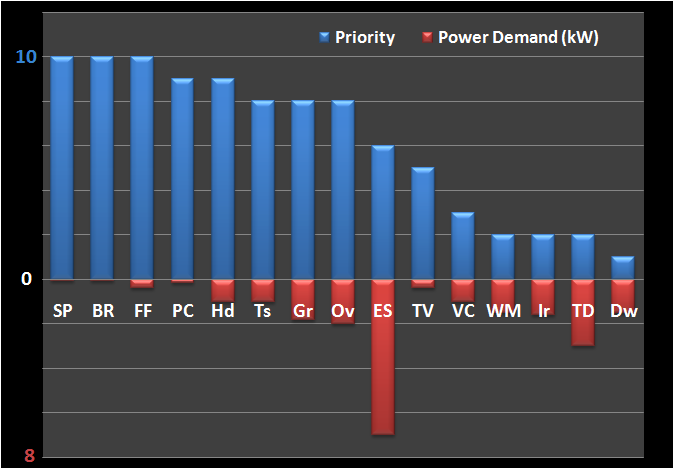
\includegraphics[width=80mm]{results.png}\\
  \caption{Simulating the order for powering the objects from the left to right}\label{fig2}
\end{figure}

For a power budget of 23 kw, all objects shall be powered, because the total demand of the objects of $O$ is $22.365<23$. If the power budget would be 10 kW, objects would be powered in order from left to right as shown in the Figure \ref{fig2}. Objects SP to Ov would get powered straight away. Their demand is 6.356, therefore the remaining power is 3.635. Object ES is skipped as its demand is larger than the remaining power resource, and objects TV, VC, WM will be powered (their demand is 2.9). The remaining power 0.735 cannot satisfy any of the remaining objects, therefore the remaining power budget is waisted and objects ES, Ir, TD and Dw are not powered.


\section{Discussion, Conclusion and Further Work} \label{discussion}
In Section \ref{intro} we described our interest and motivation for the paper. We also presented an overview of the framework specification we were to present and pointed out strengths and weaknesses of our approach. In the further section, Section \ref{problem}, we have described a mathematical model of the IoT, we developed four algorithms for the model, and in the last part, we developed a proof of correctness for main properties of the model/framework.

The present work has attempted to describe a framework for a real time resource-constrained problem. However, dealing with a complex system (IoT), we made a series of assumptions attempting to simplify it.

Further work in this area of research can explore issues that have not been considered in this paper, including:
\begin{itemize}
    \item having objects that can change their power demands in time (e.g. thinking of a hairdryer machine, normally has few levels of power),
    \item explore what happens when the power supplier is varying the available power resource,
    \item and nonetheless, creating applying the framework in real life with the help of simulation.
\end{itemize}

\bibliographystyle{IEEEtran}
%\bibliographystyle{abbrv}
\bibliography{IEEEabrv,../References}


%=======================================
%	End Document
%=======================================
%\balancecolumns
\end{document}
